%%%%%%%%%%%%%%%%%%%%%%%%%%%%%%%%%%%%%%%%%%%%%%%%%%%%%%%%%%%%%%%%%%%%%%%%%%%%%%%%
% Template for USENIX papers.
%
% History:
%
% - TEMPLATE for Usenix papers, specifically to meet requirements of
%   USENIX '05. originally a template for producing IEEE-format
%   articles using LaTeX. written by Matthew Ward, CS Department,
%   Worcester Polytechnic Institute. adapted by David Beazley for his
%   excellent SWIG paper in Proceedings, Tcl 96. turned into a
%   smartass generic template by De Clarke, with thanks to both the
%   above pioneers. Use at your own risk. Complaints to /dev/null.
%   Make it two column with no page numbering, default is 10 point.
%
% - Munged by Fred Douglis <douglis@research.att.com> 10/97 to
%   separate the .sty file from the LaTeX source template, so that
%   people can more easily include the .sty file into an existing
%   document. Also changed to more closely follow the style guidelines
%   as represented by the Word sample file.
%
% - Note that since 2010, USENIX does not require endnotes. If you
%   want foot of page notes, don't include the endnotes package in the
%   usepackage command, below.
% - This version uses the latex2e styles, not the very ancient 2.09
%   stuff.
%
% - Updated July 2018: Text block size changed from 6.5" to 7"
%
% - Updated Dec 2018 for ATC'19:
%
%   * Revised text to pass HotCRP's auto-formatting check, with
%     hotcrp.settings.submission_form.body_font_size=10pt, and
%     hotcrp.settings.submission_form.line_height=12pt
%
%   * Switched from \endnote-s to \footnote-s to match Usenix's policy.
%
%   * \section* => \begin{abstract} ... \end{abstract}
%
%   * Make template self-contained in terms of bibtex entires, to allow
%     this file to be compiled. (And changing refs style to 'plain'.)
%
%   * Make template self-contained in terms of figures, to
%     allow this file to be compiled. 
%
%   * Added packages for hyperref, embedding fonts, and improving
%     appearance.
%   
%   * Removed outdated text.
%
%%%%%%%%%%%%%%%%%%%%%%%%%%%%%%%%%%%%%%%%%%%%%%%%%%%%%%%%%%%%%%%%%%%%%%%%%%%%%%%%

\documentclass[letterpaper,twocolumn,10pt]{article}
\usepackage{usenix_2020_09}

% to be able to draw some self-contained figs
\usepackage{tikz}
\usepackage{amsmath}
%\usepackage[demo]{graphicx}
\usepackage{caption}
\usepackage{subcaption}
\PassOptionsToPackage{hyphens}{url}\usepackage{hyperref}

% inlined bib file
\usepackage{filecontents}

% add algorithm
\usepackage{algorithm}
\usepackage{algpseudocode}
\usepackage[colorinlistoftodos]{todonotes}
\usepackage{comment}


%-------------------------------------------------------------------------------
\begin{document}
%-------------------------------------------------------------------------------

%don't want date printed
\date{}

% make title bold and 14 pt font (Latex default is non-bold, 16 pt)
\title{\Large \bf Measuring Context Switches in Serverless Environments }

%for single author (just remove % characters)
\author{
{\rm Elaine Yao}\\
elainedv111@gmail.com
% copy the following lines to add more authors
% \and
% {\rm Name}\\
%Name Institution
} % end author

\maketitle

%-------------------------------------------------------------------------------
% \begin{abstract}
%-------------------------------------------------------------------------------
% Todo


% \end{abstract}


%-------------------------------------------------------------------------------
\section{Introduction}
%-------------------------------------------------------------------------------
% Serverless functions are scheduled by the provider, and charged for actual execution time (different)

% Provider wants to run more function invocaion(performance) at the same hardware-> lowest resource cost, and increasing execution time -> more money 
% Previous work shows . Part of the cycles are spent in context switching.(def cite)
% cnsw is .. ->  .. requires... -> And we want to measure 

% Prior works has focused on 1)  ... 2)....   
% we first analyzes the triggers to context switch in Linus systems, 
%In contrast, the cnsw in cloud involves more including ... and needs a more comprehensive ...


In this work, we aim to answer the following research questions:
\begin{enumerate}
	\item 
	\item 
	
\end{enumerate}


% \section{Background}
% \subsection{Serverless environment}

\subsection{Context switches}


\section{Methodology}



\subsection{Challenges}
Measuring the context switch time in serverless functions has several challenges:
\begin{itemize}
	\item [C1] Characteristics of context switch in serverless environments
	Context switch is triggered differently in serverless functions compared to in traditional operating systems as it's scheduled by the cloud provider.
	And the service provider has the tendency to trigger more functions in the same hardware to get more profits. 
	Thus, context switch may happen not only due to performance factors like multi-threading/processing, but also provider's profit considerations.
	\item [C2] Benchmark accuracy
	As no such benchmark is provided so far, we have to analyze the factors in our own benchmark that may lead to the potential variation to golden value, 
	in order to reason about the accuracy of the measurement.
	% Variations to golden values in measurement
	\item [C3] 
\end{itemize}

\subsection{}
	To tackle \emph{C1}, we design the following experiments to analyze the factors influencing context switch in serverless environments.
	We measure the execution time elapse between two adjacent lines of code repeatedly under different configurations in serverless functions.
	Shahrad \emph{et al.} \cite{serverless-main} shows that the execution time in serverless functions is influenced by function invocation frequency, memory size and function type.
	Thus these configurations will include the function invocation rate, memory allocated.
	Theoriotically, the measured time elapse should be 0 as there is not execution between these two lines. 
	However, our initial experiments show that this is neither 0 nor a fixed value, indicating that interruption happens between these two lines
	and the time elapse changes with different configurations. 
	Although the interruption is not limited to context switch but also page faults handling or container management, 
	it can still provides insights in the influence of different configurations on context switch time in serverless environments.


\subsection{Combine various benchmarks}
	To tackle \emph{C2}, we first run our own designed benchmarks on local Linux system and compare the results with published benchmarks\cite{cs-lmbench,cs-pipes,cs-arm,cs-web},
	 ensuring the correctness of the proposed ones. Then we deploy the new benchmarks in serverless functions and compare the results. 
	 If one of the benchmarks is consistently higher or lower than others, then we'll explore the reasons and this can help us improve our accuracy.

	The previous benchmarks in context switching on Linux system mainly consider %some fa
	Our initial study to \emph{C1} finds that context switch in serverless environments will also be influenced by invocation rate and memory allocation.   

	Currently, the new benchmarks are designed as the prior benchmarks with different configurations.
	The prior benchmarks we are choosing are:
	\begin{enumerate}
		\item 
	\end{enumerate}
	Next, we'll implement these functions with different invocation rate and memory allocation setting in the cloud.

% "Based on these traditional methods, we also used pipe communication to implement frequent context switches between two processes."


\section{Experiments}
 
\subsection{Experiment setup}

\subsection{Measuring local context switches}

% Figure~\ref{fig:attack-1}.

% \begin{figure}
% 	\centering
% 	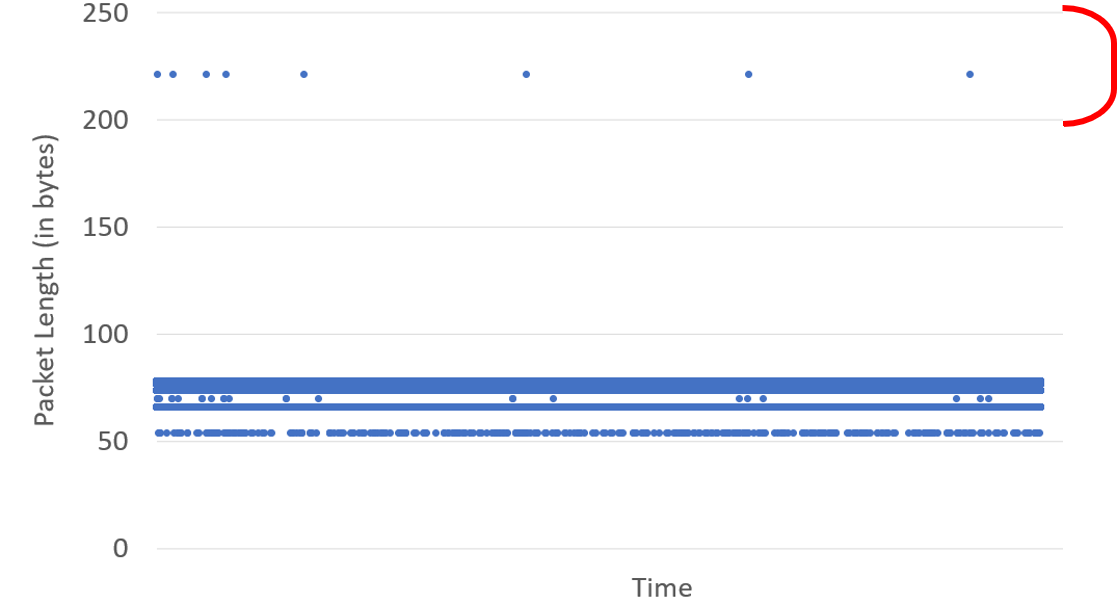
\includegraphics[width=\linewidth]{figure/attack1.png}
% 	\caption{Plot of Modbus packet lengths}
% 	\label{fig:attack-1}
% \end{figure}


\subsection{Measuring context switches in the cloud}


\section{Future work}
We plan to look at the following problems in the future.
\begin{enumerate}
    \item Implement condition variable and lmbench in python and deploy the function in the cloud.
    We aim to measure the context switches in different ways in order to improve its accuracy.
    \item Explore the factors that influence the number and the time of the context switch in serverless environment.
\end{enumerate}


\section{Related Work}
% Chen \emph{et al.}\cite{side-channel-shuo-chen} 




\bibliographystyle{plain}
\bibliography{refences}

%%%%%%%%%%%%%%%%%%%%%%%%%%%%%%%%%%%%%%%%%%%%%%%%%%%%%%%%%%%%%%%%%%%%%%%%%%%%%%%%
\end{document}
%%%%%%%%%%%%%%%%%%%%%%%%%%%%%%%%%%%%%%%%%%%%%%%%%%%%%%%%%%%%%%%%%%%%%%%%%%%%%%%%

%%  LocalWords:  endnotes includegraphics fread ptr nobj noindent
%%  LocalWords:  pdflatex acks